\chapter{Transducers}\label{chap8}

Transducers\index{Transducers} are devices that are used to convert one form of energy into another form. They convert physical quantities such as pressure, force, temperature etc. into quantities that are suitable for measurement. Transducers are extensively used in industries, medical diagnostic instruments, automobiles etc. This chapter discusses the various types of transducers, their applications, merits and demerits.

\section{Need for Transducers}\label{sec8.1}

There is a great need to sense the change in the physical parameter and convert it into a measurable quantity or to convert one form of energy into another form. Some of the examples which we see around us are as follows.
\begin{enumerate}
\item Physical parameters such as temperature, pressure, flow, density etc. need to be measured and controlled in an industry in order to obtain the product with desired specifications.

\item To measure and indicate the heart rate, blood pressure, to take ECG and EEG wave forms and to obtain the image of the internal ogran in medical science for the diagnosis of a disease.

\item Converting variation in sound into variation in electrical voltage or current and vice versa in communication systems.

\item To measure and indicate the speed, to indicate the fuel level and to turn off the indicator lamps when the steering has restored its normal position after a turn etc. in an automobile and so on. 
\end{enumerate}

In all these applications a special device called the transducer is used.

\section{Transducer}\label{sec8.2}

A transducer is a device or combination of elements which responds to the physical condition or chemical state of a substance and converts it into an output signal. A transducer converts a signal in one form of energy to another form of energy. 

The output signal from a transducer may be an electrical or mechanical parameter which can be easily measured.

If a transducer produces a mechanical nature signal as its output proportional to its input energy, it is called a mechanical transducer.

If a transducer produces an electrical signal as output in response to its input energy, it is called an electrical transducer.

A mechanical transducer needs to be cascaded with electrical transducer when an electrical output is required with non electrical input quantity as shown in Fig.~\ref{fig8.1}.
\begin{figure}[H]
\centering
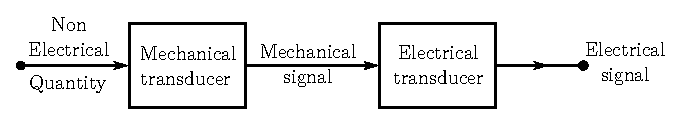
\includegraphics{chap8/fig8.1.eps}
\caption{Cascade of Mechanical and electrical transducers}\label{fig8.1}
\end{figure}

\subsection{Difference between the sensor and the transducer}\label{sec8.2.1}

A sensor\index{Sensor} is used to detect a parameter in one form and report it in another form of energy, most often an electrical signal. Intensity and luminance of a source may be measured by sensors. 

Transducer converts a signal in one form of energy to another form of energy.

\section{Classification of Transducers}\label{sec8.3}
\index{Transducer!classification of}

Transducers can be classified on the following basis.

\smallskip
\heading{(a)~ Based on the role}

Based on the role, transducers can be classified into input and output transducers.

An input transducer also known as an instrument transducer can be used as a measurement device.

An output transducer delivers force, torque, pressure or displacement as output when an electrical signal is applied as an input. It is also called as a power transducer.

\eject

\heading{(b)~ Based on the operation}

Based on the operation, transducers are classified into active and passive transducers.

Active transducers are those which accept energy from the physical quantity to be detected or measured and self generate an output that is proportional to the physical quantity. Thermocouple, piezo electric transducers, photo electric cell and photovoltaic cell are the examples of active transducers.

Passive transducers are those which accept energy from the applied power source used for measurement, and modify it suitably in accordance with variations of the physical quantity under measurement. Resistive strain gauge, thermistor, LVDT, Hall effect sensor and photo multiplier tube are examples of passive transducers.

\section{Desirable properties of a Good Transducer}\label{sec8.4}
\index{Transducer!properties of}

Following are the desirable properties of a good transducer.
\begin{enumerate}
\renewcommand{\labelenumi}{\bf\theenumi.}
\item {\bf Linearity~:} A good transducer must have a linear input - output characteristic i.e., the output should vary directly with the input.

\item {\bf Accuracy~:} A good transducer must produce a high degree of accuracy in its conversion process.

\item {\bf Repeatability (Precision)~:} A transducer must be able to produce the same output for the same input applied for a large number of times under the same operating conditions.

\item {\bf Stability and Reliability~:} A transducer must be stable and reliable in its operation i.e., the output of the transducer should not get affected by temperature, vibration and other environmental variations and also the measurement error should be minimal.

\item {\bf Dynamic Response~:} A transducer must have good dynamic response i.e., it must be able to operate uniformly and smoothly over a wide range of frequencies.

\item {\bf Ruggedness and residual deformation~:} Transducers must be rugged in their structure and operation. They must be able to withstand overloads safely.

Also a transducer must retain its original shape and structure even after long period of usage.

\item {\bf Large output and good signal quality~:} A good transducer must produce a sufficiently large output even for a small input.

Also the signal quality must be very good. This implies that the signal-to-noise ratio must be large (the output should be free from noise). 
\end{enumerate}

\section{Mechanical Transducers}\label{sec8.5}
\index{Mechanical Transducers}

Mechanical transducers\index{Transducer!mechanical transducers} are mechanical elements which are used for converting one form of energy into another form that can be measured easily.

The important mechanical quantities which are to be measured and controlled in any industry are temperature, pressure, force, torque, density, liquid level, viscosity, flow rate, displacement, velocity, acceleration, altitude and distance.

A brief description of some of the commonly used mechanical transducers is given below.

\smallskip

\heading{Spring~:}\index{Spring} Springs are used for the measurement of force. The spring gets elongated when it is subjected its a tensile force and compressed when subjected to compressive force as shown in Fig.~\ref{fig8.2}.
\begin{figure}[H]
\centering
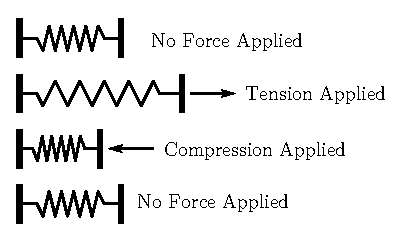
\includegraphics[scale=.86]{chap8/fig8.2.eps}
\caption{Spring Under Tension \&\ Compression}\label{fig8.2}
\end{figure}

\heading{Bellows~:}\index{Bellows} Bellows are used for the measurement of pressure. Bellows are elastic elements that convert the air pressure into displacement. The displacement is indicated by the pointer attached to the bellow as shown in Fig.~\ref{fig8.3}.
\begin{figure}[H]
\centering
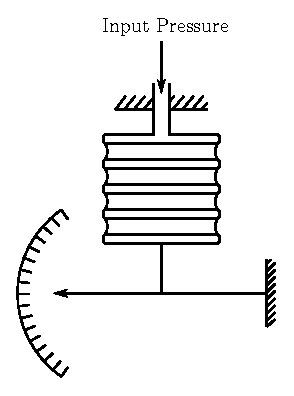
\includegraphics[scale=.86]{chap8/fig8.3.eps}
\caption{Bellow used to measure the pressure}\label{fig8.3}
\end{figure}

\heading{Bourdon tube~:}\index{Bourdon tube} Bourdon tube is used to measure the pressure. It is an elastic tube that converts air pressure into the rotary motion of the pointer which inturn indicates the pressure. Fig.~\ref{fig8.4} shows the displacement of Bourdon tube due to the applied pressure.
\begin{figure}[H]
\centering
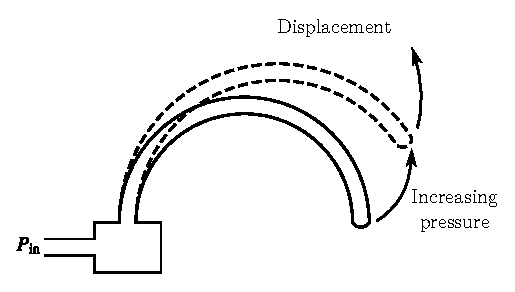
\includegraphics{chap8/fig8.4.eps}
\caption{Bourdan Tube used to measure the pressure}\label{fig8.4}
\end{figure}

\heading{Proving Rings~:}\index{Proving Rings} They are similar to springs in action. They convert applied force into displacement.

\smallskip

\heading{Thermocouple~:}\index{Thermocouple} Thermocouple is used to measure the temperature of a body. It is a device that produces electric current when one of its end is heated. The current produced is proportional to the temperature to be measured. Thermocouples are discussed in detail in Section~\ref{sec8.13}.

\smallskip

\heading{Bimetals~:}\index{Bimetals} Bimetals are used to measure the temperature. They are also called as Bimetallic strips which consists of two different metals having different coefficient of thermal expansion, joined together as shown in Fig.~\ref{fig8.5}. Upon heating the strip, both the metals expand but the expansion of one metal is lesser than that of the other. The difference in expansion results in the deflection of the bimetallic strip, which is converted into the rotary motion of the pointer that indicates the temperature.
\begin{figure}[H]
\centering
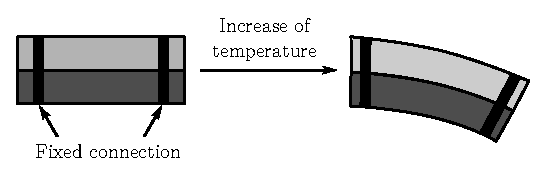
\includegraphics{chap8/fig8.5.eps}
\caption{Bimetallic strip}\label{fig8.5}
\end{figure}

\eject

\heading{Diaphram~:}\index{Diaphram} Diaphram converts the applied pressure into the displacement.

\smallskip

\heading{Manometer~:}\index{Manometer} It is used to measure pressure. The applied pressure causes the displacement of the liquid in the manometer and this displacement is used to indicate the pressure as shown in Fig.~\ref{fig8.6}.
\begin{figure}[H]
\centering
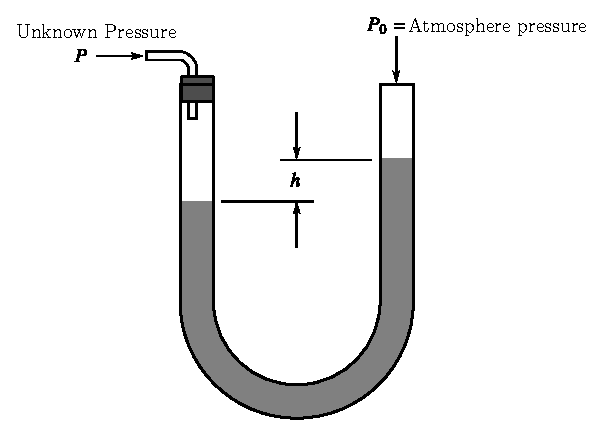
\includegraphics{chap8/fig8.6.eps}
\caption{Manometer}\label{fig8.6}
\end{figure}
Change in pressure, 
\begin{align*}
\Delta P &=(P-P_{0})\,\alpha\, h,\\
h &=\text{~ displacement of the liquid.}
\end{align*}

\heading{Hydropneumatic Transducers~:}\index{Hydropneumatic Transducers} They are used for the measurement of pressure, velocity, flow rate and force of water. Examples of hydropneumatic transducers are orifice, venturi, vanes, pitot tube and turbines. 

\section{Strain Gage}\label{sec8.6}

A strain gage\index{Strain gage} is a device used to measure strain on an object. The strain gage makes use of the property that electrical conductance depends on the dimensions of the conductor.
\begin{itemize}
\itemsep=0pt
\item[$\bullet$] When an electrical conductor is stretched within the limits of its elasticity, it becomes narrower and longer resulting in an increase in its resistance.

\item[$\bullet$] Conversely, when a conductor is compressed such that it does not buckle, it will broaden and shorten resulting in the decrease in its resistance. 

\item[$\bullet$] From the measured electrical resistance of the strain gage, the amount of applied stress may be inferred. The change in resistance can be measured using a wheat stone bridge.
\end{itemize}

A Typical strain gage consists of a long, thin conductive strip, arranged in a zig-zag pattern on an insulating flexible support as shown in Fig.~\ref{fig8.7}. The conducting strip is usually made of nichrome and the insulating support is an impregnated paper dipped in insulating varnish. 
\begin{figure}[H]
\centering
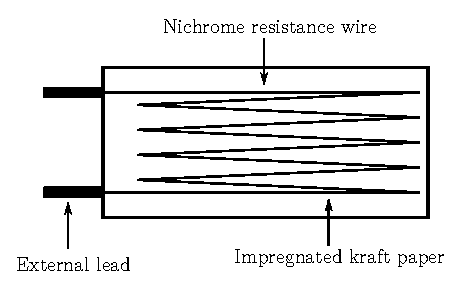
\includegraphics[scale=.9]{chap8/fig8.7.eps}
\smallskip
\caption{Resistance strain gage}\label{fig8.7}
\end{figure}

\subsection{Applications of strain gage}\label{sec8.6.1}

Strain gage is used in the
\begin{itemize}
\itemsep=2pt
\item[$\bullet$] Experimental stress analysis of machines and structures.

\item[$\bullet$] Construction of the transducers used in the measurement of force, torque, pressure, temperature, acceleration etc.
\end{itemize}

\section{Passive electrical transducers}\label{sec8.7}
\index{Transducer!passive electrical}

The three passive elements in an electrical circuit are resistor, inductor and capacitor. Passive transducers produce the change in resistance, inductance or capacitance in response to the change in the physical quantity to be measured. Accordingly we have the following three types of passive transducers.
\begin{enumerate}
\itemsep=2pt
\item Resistive transducer\qquad 2.~ Inductive transducer\qquad 3.~ Capacitive transducer
\end{enumerate}

\section{Resistive Transducers}\label{sec8.8}

A resistive transducer\index{Resistive transducer} produces resistance variation in accordance with the physical quantity sensed. 

The $dc$ resistance $R$ of a conducting wire is given by
\begin{align}
R &= \frac{\rho l}{a}\label{eq8.1}\\[1pt]
\text{where}\qquad \rho &= \text{specific resistivity in $\Omega-\text{m}$}\notag\\[1pt]
l &= \text{conductor length in m}\notag\\[1pt]
a &= \text{area of cross section in m$^{2}$}\notag
\end{align}

The change in the resistance value occurs when the externally applied stimulus affects either the dimensions ($l$ and $a$) or the resistivity $(\rho)$ of the resistive element. When the resistive elements are subjected to pressure, force or torque, the dimensional change occurs. Strain gages work on this principle. They can be used to measure displacement, force and pressure.

The resistivity of a material changes with temperature and composition of the material. Resistance thermometers makes use of this principle and they are used in temperature measurement.\\[-20pt]

\subsection{Resistance Thermometer}\label{sec8.8.1}
\begin{itemize}
\itemsep=0pt
\item[$\bullet$] In resistance thermometer,\index{Resistance thermometer} the change in temperature is measured in terms of the change in resistance.

\item[$\bullet$] The resistive element is made of solid material, a metal, metallic alloy or a semiconductor compound.

\item[$\bullet$] In metals, resistivity increases with temperature whereas it decreases in semiconductors and insulators.

\item[$\bullet$] In metals, the length also increases with temperature in addition to increase in resistivity. Hence the change in resistance is due to both change in length and resistivity.

\item[$\bullet$] The resistance $R_{T}$ of a resistance thermometer at any temperature is given by
\begin{align}
R_{T} &=R_{0}(1+\alpha T)\label{eq8.2}\\[1pt]
\text{where,}\qquad R_{0} &= \text{Resistance at $0^{\circ}$C}\notag\\[1pt]
                    T &= \text{Temperature in $^{\circ}$C}\notag\\[1pt]
               \alpha &= \text{Temperature co-efficient of resistance}\notag\\[1pt]
               \alpha &= \frac{1}{\Delta T}\cdot \frac{\Delta R}{R_{0}}\label{eq8.3}
\end{align}
\vfill\eject
~\phantom{a}
\vskip -1cm
\begin{flalign*}
&\text{where},&\Delta T &= \text{Change in temperature in $^{\circ}$C}\hspace{4cm}\\
&& \Delta R &= \text{Change in resistance}\\[-.8cm]
\end{flalign*}

\itemsep=1pt
\item[$\bullet$] Fig.~\ref{fig8.8} shows the wire resistance thermometer.
\begin{figure}[H]
\centering
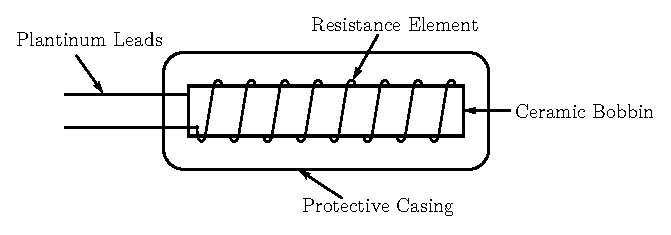
\includegraphics[scale=.85]{chap8/fig8.8.eps}
\caption{Wire resistance thermometer}\label{fig8.8}
\end{figure}

\item[$\bullet$] It consists of a length of a fine coiled wire wrapped around a ceramic, mica or a glass base. The base also serves as the mount for the coil.

\item[$\bullet$] The element is usually quite fragile and therefore it is enclosed in a protective tube of pyrex glass, porcelain, quartz or nickel. 

\item[$\bullet$] The materials used for the construction of resistive thermometer are platinum, nickel and copper. Platinum is the most commonly used material.

\item[$\bullet$] For temperature measurement, the resistance thermometer is used as one arm of the wheat stone bridge as shown in Fig.~\ref{fig8.9}.
\begin{figure}[H]
\centering
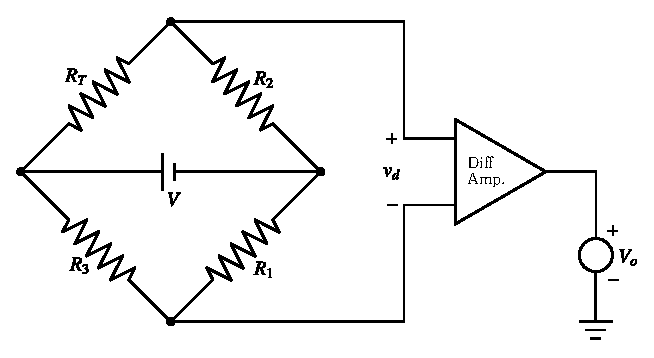
\includegraphics[scale=.8]{chap8/fig8.9.eps}
\caption{Wheat stone bridge to measure change\break in $R_{T}$}\label{fig8.9}
\end{figure}

\item[$\bullet$] Whenever $R_{T}$ changes due to change in temperature the bridge is imbalanced, generating a voltage $V_{d}$ which is amplified and indicated.
\end{itemize}

\subsection{Advantages of resistance thermometer}\label{sec8.8.2}

Following are the advantages of resistance thermometers:
\begin{itemize}
\item[$\bullet$] It is one of the most accurate temperature sensors.

\item[$\bullet$] It provides excellent stability and precision. 

\item[$\bullet$] It has a high linear temperature-resistance characteristic.

\item[$\bullet$] It has faster response than thermistors. 
\end{itemize}

\subsection{Disadvantages}\label{sec8.8.3}

The disadvantages of resistance thermometer are as follows.
\begin{itemize}
\item[$\bullet$] It has lower sensitivity.

\item[$\bullet$] Bigger in size than thermistors.

\item[$\bullet$] Higher cost.

\item[$\bullet$] Possibility of self heating.
\end{itemize}

\section{Thermistor}\label{sec8.9}

The name thermistor\index{Thermistor} is coined from the words thermal and resistor. Thermistor is a two terminal semiconductor slab which has negative temperature coefficient (NTC) of resistance i.e., its resistance decreases with increase in temperature.

Fig.~\ref{fig8.10} shows the temperature-resistance characteristic of a thermistor.
\begin{figure}[H]
\centering
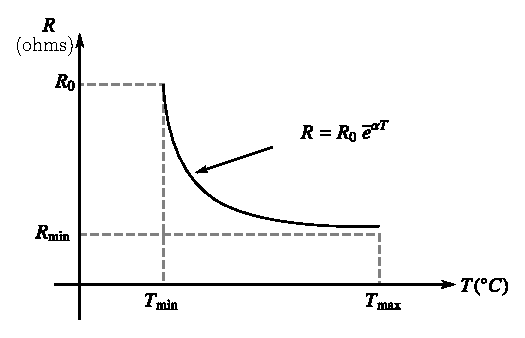
\includegraphics[scale=.9]{chap8/fig8.10.eps}
\caption{Temperature-resistance characteristic of thermistor}\label{fig8.10}
\end{figure}

The resistance decreases exponentially according to the equation,
\begin{equation}
R=R_{0}\,e^{-\alpha T}\label{eq8.4}
\end{equation}
where
\begin{quote}
$R_{0}=$ maximum resistance corresponding to minimum temperature.

$\alpha=$ a constant dependent on the thermistor type.
\end{quote}

\subsection{Construction of thermistors}\label{sec8.9.1}
\begin{itemize}
\item[$\bullet$] Thermistors are made up of oxides of metals such as those of manganese, nickel, cobalt, iron, copper and titanium.

\item[$\bullet$] To construct thermistors, two or more metal oxides are mixed using suitable binding materials.

\item[$\bullet$] The mixture is then formed into the desired shape, dried and sintered at a high temperature.

\item[$\bullet$] Each sintered piece is then hermetically sealed in a glass enclosure to prevent air and humidity from reacting with the thermistor material.

\item[$\bullet$] Fig.~\ref{fig8.11} shows different structures of thermistors.
\begin{figure}[H]
\centering
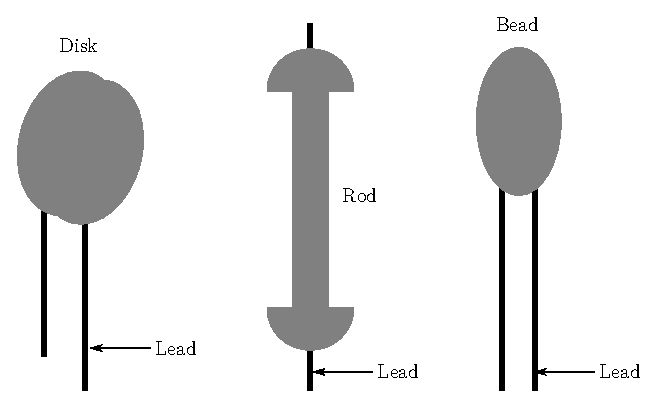
\includegraphics{chap8/fig8.11.eps}
\caption{Structures of thermistors}\label{fig8.11}
\end{figure}
\end{itemize}

\subsection{Applications of Thermistors}\label{sec8.9.2}

Thermistors are used in the measurement of
\begin{itemize}
\item[$\bullet$] Temperature

\item[$\bullet$] Flow and pressure

\item[$\bullet$] Liquid level

\item[$\bullet$] Voltage and power

\item[$\bullet$] Vaccum

\item[$\bullet$] Thermal conductivity
\end{itemize}

\subsection{Advantages of thermistor}\label{sec8.9.3}

The advantages of thermistor are:
\begin{itemize}
\item[$\bullet$] Small size and low cost

\item[$\bullet$] Fast response over narrow temperature range

\item[$\bullet$] Good sensitivity in negative temperature coefficient region
\end{itemize}

\subsection{Disadvantages of thermistor}\label{sec8.9.4}

The disadvantages of thermistor are:
\begin{itemize}
\item[$\bullet$] The temperature - resistance characteristic is non linear

\item[$\bullet$] Not suitable for wide range of temperature measurement
\end{itemize}

\section{Resistive displacement transducers}\label{sec8.10}
\index{Resistive displacement transducers}

\begin{itemize}
\item[$\bullet$] The resistive displacement\index{Transducer!resistive displacement} transducers are used to measure the linear displacement or the angular displacement.

\item[$\bullet$] The resistive element is provided with a movable contact, which moves and causes a change in resistance, whenever there is a displacement.
\end{itemize}

Fig.~\ref{fig8.12} shows a potentiometer used as a resistive displacement transducer to measure the linear displacement.
\begin{figure}[H]
\centering
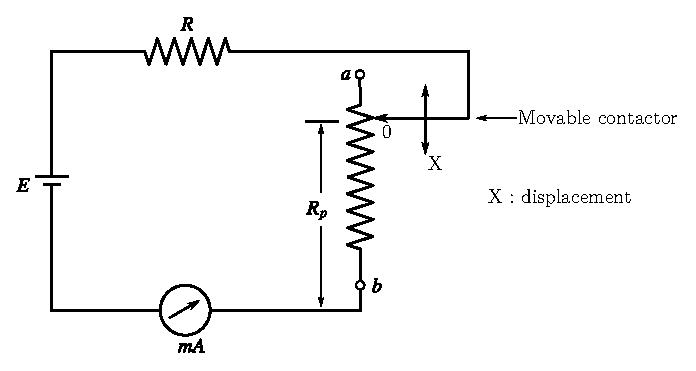
\includegraphics[scale=.9]{chap8/fig8.12.eps}
\caption{Resistive transducer to measure linear displacement}\label{fig8.12}
\end{figure}

The displacement causes the movable contact to move downward. This reduces the potentiometer resistance $R_{p}$ which results in an increase in ammeter current. Note that the change in current is proportional to the change in resistance $R_{p}$ which in turn is proportional to the displacement.

For angle measurement, the resistor element is in circular form and the contactor is rotatable as shown in Fig.~\ref{fig8.13}.
\begin{figure}[H]
\centering
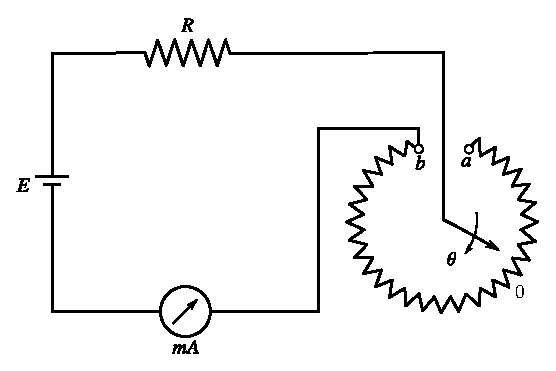
\includegraphics[scale=.9]{chap8/fig8.13.eps}
\caption{Resistive transducer to measure angular displacement}\label{fig8.13}
\end{figure}

\section{Inductive transducers}\label{sec8.11}
\index{Transducer!inductive transducers}

In inductive transducers\index{Inductive transducers} the self inductance of a coil or mutual inductance of a pair of coils is made to vary in relation to the physical quantity to be measured. Linear variable differential transformer (LVDT) is an example of inductive transducer.\\[-20pt]

\subsection{The Linear Variable Differential Transformer (LVDT)}
\index{Linear Variable Differential Transformer (LVDT)}

Fig.~\ref{fig8.14} shows the construction of LVDT.
\begin{figure}[H]
\centering
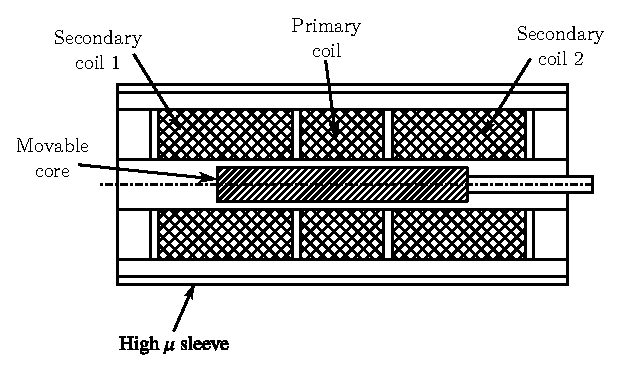
\includegraphics{chap8/fig8.14.eps}
\caption{Construction of LVDT}\label{fig8.14}
\end{figure}

It consists of a plastic cylindrical former on which three coils are wound. The middle coil is the primary and two identical secondary coils are wound symmetrically on either side of the primary coil and away from the centre. The secondary coils are connected in series opposition so that output voltage will be the difference between the individual voltages induced in the secondary coils;
hence the name differential transformer. 

A ferrite rod is kept inside the plastic former which acts as the core of the transformer and it is free to move inside the former. When an $ac$ voltage is applied to the primary coil, voltages are induced in the secondary coils whose value depends on the core position. The displacement of the core is caused by the physical quantity under measurement. Let us consider the following cases.

\smallskip
\heading{(a) Core in the centre position} 
\smallskip

When the core is in the centre position, both secondary coils will have the same amount of flux linkage and hence same induced emfs. i.e., $V_{01}=V_{02}$ and hence
$$
V_{0}=V_{01}-V_{02}=0
$$

\eject

This is illustrated in Fig.~\ref{fig8.15}.
\begin{figure}[H]
\centering
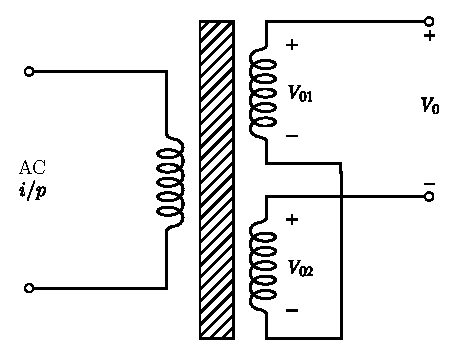
\includegraphics{chap8/fig8.15.eps}
\caption{Core in the centre position}\label{fig8.15}
\end{figure}

\heading{(b) Core towards secondary coil 1 and away from coil 2}

In this case, the secondary coil 1 has more flux linkage than coil 2. Hence more emf is induced in coil 1 than in coil 2 i.e., $V_{01}>V_{02}$.
$$
\therefore~ V_{0}=V_{01}-V_{02}\quad\text{is positive.}
$$
This is illustrated in Fig.~\ref{fig8.16}.
\begin{figure}[H]
\centering
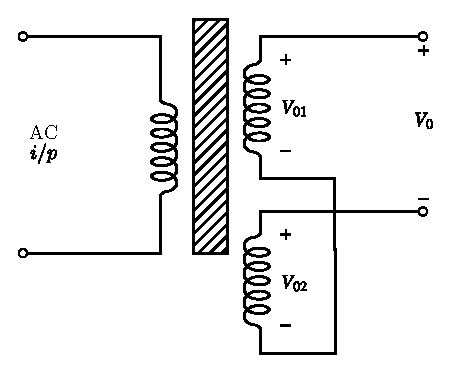
\includegraphics{chap8/fig8.16.eps}
\caption{Core towards secondary coil 1}\label{fig8.16}
\end{figure}

\eject

\heading{(c)~ Core towards secondary coil 2 and away from coil 1}

In this case, the secondary coil 2 has more flux linkage than coil 1. Hence more emf is induced in coil 2 than in coil 1. i.e., $V_{0_2}>V_{0_1}$.
$$
\therefore\quad V_{0}=V_{01}-V_{02}\quad\text{is negative}
$$
This is illustrated in Fig.~\ref{fig8.17}.
\begin{figure}[H]
\centering
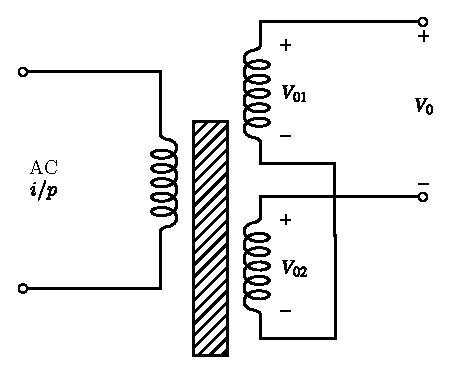
\includegraphics[scale=.9]{chap8/fig8.17.eps}
\caption{Core towards secondary coil 2}\label{fig8.17}
\end{figure}

The transfer characteristic of LVDT is shown in Fig.~\ref{fig8.18}. Note that the characteristic is fairly linear.
\begin{figure}[H]
\centering
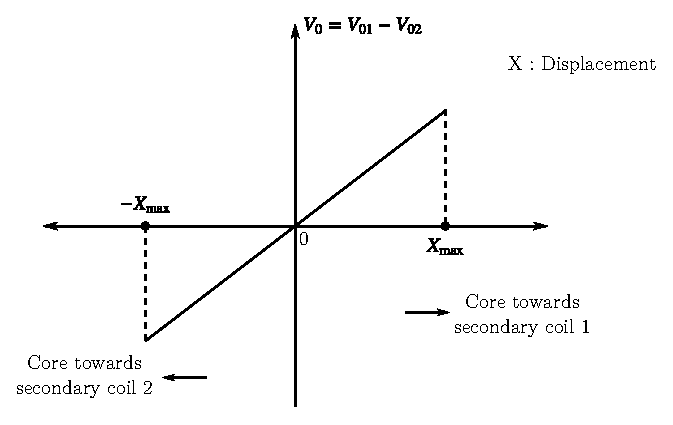
\includegraphics[scale=.9]{chap8/fig8.18.eps}
\caption{Transfer characteristic of LVDT}\label{fig8.18}
\end{figure}

The output voltage is the difference between (Differential) the voltages of secondary coils. The output voltage varies linearly with the position of the core. Hence the name:

Linear Variable Differential Transformer.

\subsection{Applications of LVDT}\label{sec8.11.1}

Following are the applications of LVDT.
\begin{itemize}
\item[$\bullet$] Measurement of force

\item[$\bullet$] Measurement of weight

\item[$\bullet$] Measurement of velocity, acceleration

\item[$\bullet$] Sensing vibrations
\end{itemize}

\section{Active Electrical Transducers}\label{sec8.12}
\index{Electrical Transducers}

The popular Active electrical transducers are
\begin{itemize}
\item[(a)] Thermoelectric transducers

\item[(b)] Piezo electric transducers and

\item[(c)] photo electric transducers
\end{itemize}

\section{Thermoelectric Transducers}\label{sec8.13}
\index{Thermoelectric Transducers}

Thermocouple\index{Thermocouple} is a thermoelectric transducer, which converts thermal energy into electrical energy. It consists of two wires of different metals, joined together to form two junctions as shown in Fig.~\ref{fig8.19}.

One of the two junctions is called the hot junction and the other the cold junction. Cold junction is called the reference junction. The behaviour of a thermocouple is governed by the following three phenomena.
\begin{itemize}
\item[(a)] Seebeck effect

\item[(b)] Peltier effect

\item[(c)] Thomson effect
\end{itemize}

\begin{figure}[H]
\centering
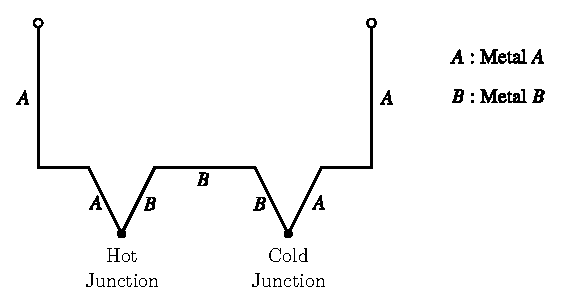
\includegraphics{chap8/fig8.19.eps}
\caption{Thermo couple}\label{fig8.19}
\end{figure}

\subsection{Seebeck Effect}\label{sec8.13.1}
\index{Seeback Effect}

If the two junctions formed by two dissimilar metals of a thermocouple are maintained at different temperatures, an emf developes between the open ends. An electric current flows if the circuit is closed by connecting the two open ends. This phenomenon in which the temperature gradient between two junctions results in an emf or electric current is called Seebeck effect or thermoelectric effect. The emf or the current depends on the temperature difference between the two junctions.

Fig.~\ref{fig8.20} illustrates the Seebeck effect.
\begin{figure}[H]
\centering
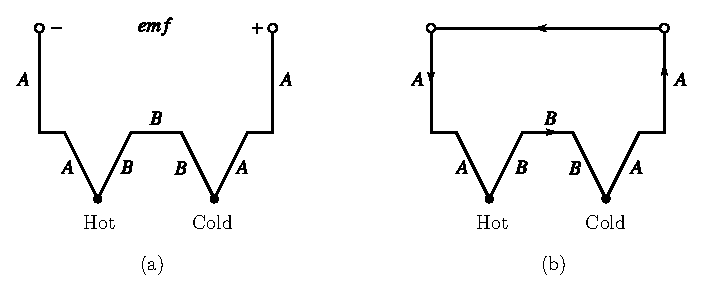
\includegraphics{chap8/fig8.20.eps}
\caption{Seebeck effect}\label{fig8.20}
\end{figure}
\begin{quote}
$A$~: Copper

$B$~: Iron
\end{quote}

If metal $A$ is of copper and metal $B$ is of iron, then the current flows from copper to iron at the hot junction and from iron to copper at the cold junction.

A few other combinations of metal $A$ and metal $B$ are listed in Table~\ref{tab8.1}.
\begin{table}[H]
\tabcolsep=6pt
\renewcommand{\arraystretch}{1.1}
\begin{tabular}{|c|c|}
\hline
{\bf Metal \boldmath$A$} & {\bf Metal \boldmath$B$}\\
\hline
Bismuth & Copper\\
Constantan & Copper\\
Chromel & Alumel\\
Copper & Zinc\\
\hline
\end{tabular}
\caption{Few combinations of metal $A$ and metal $B$}\label{tab8.1}
\end{table}

\subsection{Peltier Effect}\label{sec8.13.2}
\index{Peltier Effect}

{\em When an electric current is passed through two dissimilar metals connected to form a thermocouple, heat is evolved at one junction and absorbed at the other junction. The absorption and evolution of heat depends on the direction of flow of current.}

Peltier effect is the reverse phenomenon of Seebeck effect. Fig.~\ref{fig8.21} illustrates the peltier effect.
\begin{figure}[H]
\centering
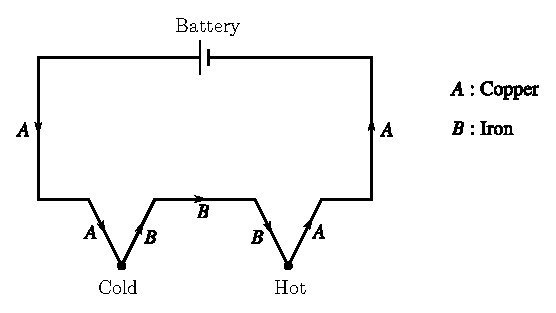
\includegraphics[scale=.95]{chap8/fig8.21.eps}
\caption{Peltier effect}\label{fig8.21}
\end{figure}

It is observed that, a temperature rise occurs at the junction, where the current passes from iron to copper, and a temperature drop occurs at the junction where the current passes from copper to iron. The amount of heat liberated or absorbed is proportional to the quantity of current that passes through the junction.

Peltier coefficient is defined as the amount of heat energy absorbed or evolved due to peltier effect at the junction of two dissimilar metals when one columb of charge passes through the junction.

Peltier effect is entirely reversible in nature.

\vfill\eject

\subsection{Thomson Effect}\label{sec8.13.3}
\index{Thomson Effect}
\begin{itemize}
\item[$\bullet$] Thomson effect is related to the emf that devolopes between two parts of a single metal when they are at different temperature.

\item[$\bullet$] Thus Thomson effect is the absorption or evolution of heat along a conductor when current passes through it, when one end of the conductor is hot and the other end is cold.

\item[$\bullet$] When current flows through a copper conductor having thermal gradient (temperature difference), heat is liberated at any point when the current is in the same direction as the heat flow, while the heat is absorbed when the current flows in the direction opposite to the flow of heat.

\item[$\bullet$] In case of iron, heat is absorbed at any point when the current flows in the direction of heat flow, while the heat is liberated, when the current flows in the direction opposite to the flow of current.

\item[$\bullet$] Thomson effect is also a reversible effect.
\end{itemize}

\subsection{Applications of Thermocouple}\label{sec8.13.4}

Some of the important applications of thermocouple are as follows.
\begin{itemize}
\item[$\bullet$] In steel industry to monitor temperature.

\item[$\bullet$] In gas-fed heating appliances to produce safety.

\item[$\bullet$] Measurement of the intensity of incident radiation.

\item[$\bullet$] In thermoelectric refrigerator or generator.
\end{itemize}

\section{Piezo-Electric Transducer}\label{sec8.14}
\index{Piezo-Electric Transducer}

Piezo-Electricity means press and generate electricity. Piezo-electricity is the ability of certain crystals and ceramics to produce electric charges when mechanical stress is applied across them in certain specified orientations. The accumulation of charges on the material surfaces will inturn give rise to a voltage across the cross section of the material.

\smallskip

The piezo-electric effect is direction sensitive. The polarity of voltages produced for tension and compression are opposite as shown in Fig.~\ref{fig8.22}.

\begin{figure}[H]
\centering
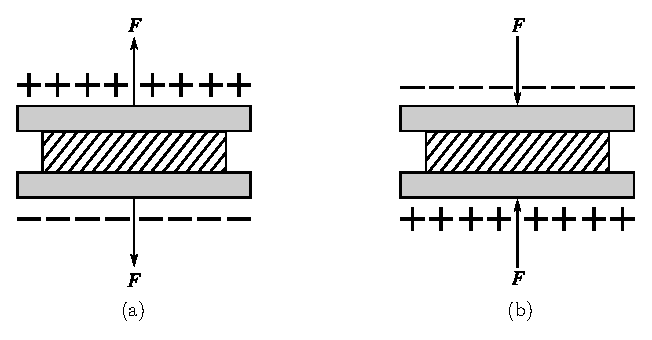
\includegraphics{chap8/fig8.22.eps}
\caption{Piezo-electric material under (a) Tension (b) Compression}\label{fig8.22}
\end{figure}

The Piezo-electric effect is reversible, that is materials exhibiting piezo-electric effect also exhibit the property of electrostriction; i.e., production of mechanical stress on application of an electric field.

\smallskip
The materials exhibiting the piezo-electric phenomenon are quartz, Rochelle salt, tourmaline, Ammonium Dihydrogen phosphate (ADP), Lithium sulphate (LS) and Di potassium Tartrate (DKT). The necessary condition for the piezo-electric effect is the absense of a centre-of-symmetry in the crystal structure.

\smallskip
A Piezo electric crystal operates in the following modes.
\begin{itemize}
\item[(a)] thickness expander mode

\item[(b)] length expander mode

\item[(c)] thickness shear mode

\item[(d)] face shear mode
\end{itemize}
The modes are based on the direction of the force applied.

\smallskip
Metal electrodes are plated onto selected faces of the pieze-electric material so that, lead wires can be attached for bringing in or leading out the electric charge. The arrangement forms plates and the piezo-electric material acting as the dielectric. 

\smallskip
The applied mechanical force generates a charge which inturn give rise to a voltage as given by the basic equation, $V=Q/C$.

\smallskip
Fig.~\ref{fig8.23} shows the piezo-electric crystal operating in thickness expansion mode.
\begin{figure}[H]
\centering
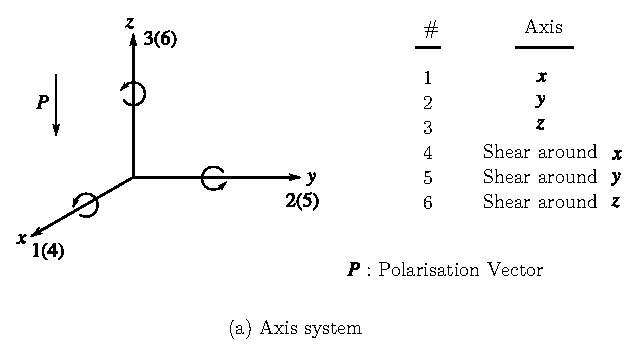
\includegraphics{chap8/fig8.23a.eps}

\bigskip
\bigskip
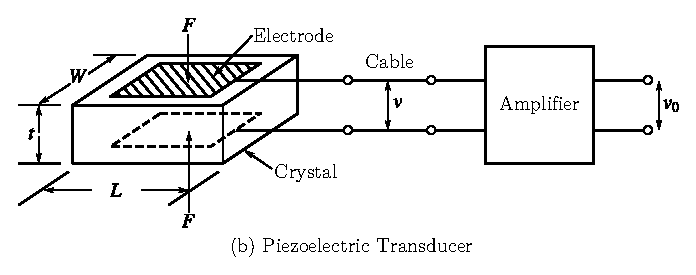
\includegraphics{chap8/fig8.23b.eps}

\caption{(a) Axis system (b) Piezoelectric Transducer}\label{fig8.23}
\end{figure}


\subsection{Advantages of Piezo-electric Transducers}\label{sec8.14.1}

The advantages of Piezo-electric transducers are
\begin{itemize}
\item[$\bullet$] Smaller in size

\item[$\bullet$] High natural frequency

\item[$\bullet$] High sensitivity

\item[$\bullet$] Linearity

\item[$\bullet$] Wide measuring range and polarity sensitivity
\end{itemize}


\eject

\subsection{Applications of Piezo-electric Transducers}\label{sec8.14.2}

The Piezo-electric transducers are used in the measurement of
\begin{itemize}
\itemsep=0pt
\item[$\bullet$] force

\item[$\bullet$] pressure

\item[$\bullet$] acceleration

\item[$\bullet$] torque

\item[$\bullet$] strain

\item[$\bullet$] amplitude of vibration
\end{itemize}
They are used in
\begin{itemize}
\item[$\bullet$] microphones as sound-to-electrical converter 

\item[$\bullet$] generation of ultrasonic frequencies

\item[$\bullet$] gas lighters
\end{itemize}

\section{Photo Electric Transducers}\label{sec8.15}
\index{Photo Electric Transducers}

When light falls on the surface of low-work function materials like cesium, electrons are emitted. This property is known as photo electricity. Work function is the amount of energy required to liberate a fermi-level electron from the surface of a metal. Fermi-level is the energy that an election can occupy at zero kelvin.

Fig.~\ref{fig8.24} illustrates photo-electric emission. 
\begin{figure}[H]
\centering
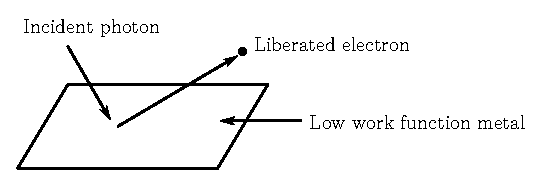
\includegraphics{chap8/fig8.24.eps}
\caption{Photo electric emission}\label{fig8.24}
\end{figure}

When the light energy (photon) interacts with an electron bound on a metal surface, the entire quantum energy is converted into kinetic energy of the election. This kinetic energy accelerates the electrons to move and results in the current flow. We have the following types of transducers which make use of photo electric effect.
\begin{itemize}
\item[(a)] Photo-emissive transducers

\item[(b)] Pho-voltaic transducers and

\item[(c)] Photo-conductive transducers 
\end{itemize}

Photo-emissive transducer consists of a semi cylindrical cathode which is coated with a photo-emissive material and an anode which is a thick metallic wire, both enclosed in an evacuated glass tube. When light is made to fall on the cathode, electrons are emitted from its surface. Under positive voltage, the anode attracts  these electrons and the anode current starts flowing. This current is proportional to the intensity of the incident light.

A photo-voltaic transducer (photo-voltaic cell) generates a potential when light falls on it. Basically, it is a $p$-$n$ junction doide with a window on the top for allowing optical radiation. Photo transistors and photo diodes functions in both photo-voltaic and photo-emissive modes.

When light or heat energy falls on a semiconductor surface, covalent bonds start breaking due to the incident energy. The rise in the number of electron hole pair is exponential. Hence the resistance of the material decreases exponentially. Cadmium sulphide (CdS) is the most widely used photo conductive material and it is popularly known as the light dependent resistor (LDR).

\subsection{Applications of Photo-Electric Transducers}\label{sec8.15.1}

{\em Photo voltaic transducers are used in}
\begin{itemize}
\item[$\bullet$] Power stations for generating electrical power

\item[$\bullet$] Solar vehicles 

\item[$\bullet$] Space crafts

\item[$\bullet$] Rural electrification 

\item[$\bullet$] Buildings for power generation for lighting purpose.

\item[$\bullet$] Solar lamps, LCDS etc.
\end{itemize}
Photo emissive transducers are used to measure the intensity of light.

Photo conductive transducers are used in
\begin{itemize}
\item[$\bullet$] Industry for object counting

\item[$\bullet$] Measuring instruments for event counting

\item[$\bullet$] Counting the number of persons entered into or exited out of an hall or auditorium

\item[$\bullet$] Optical communication systems etc.
\end{itemize}

